\chapter{Implementation}
\label{Chapter4}
\section{Technologies Used}
The implementation of the split key wallet protocol and mobile authenticator for the Züs platform involves the following technologies:
\begin{itemize}
\item Programming Languages: The core components of the system are implemented using Golang and Solidity programming languages.
\item Cryptographic Libraries: The BLS signature scheme is implemented using the Apache Milagro Cryptographic Library (AMCL), which provides efficient implementations of pairing-based cryptography.
\item Mobile Development Framework: The mobile authenticator is developed using the native Android, iOS and electron framework, enabling support for iOS, Android and Desktop devices.
\item Secure Storage: The key components and sensitive data are stored securely using hardware-backed keystores, such as the Secure Enclave on iOS and the Keystore on Android.
\end{itemize}
\section{Smart Contract Development}
The Züs platform utilizes smart contracts to facilitate decentralized storage and cryptocurrency transactions. The split key wallet protocol is integrated into the existing smart contract infrastructure. The main modifications include:
\begin{itemize}
\item Signature Verification: The smart contracts are updated to support the verification of BLS signatures, ensuring the integrity of transactions.
\item Key Management: The smart contracts handle the registration and management of public keys associated with the split key wallets.
\end{itemize}
\section{Wallet Integration}
The split key wallet protocol is integrated into the existing Züs wallet implementation. The main changes include:
\begin{itemize}
\item Key Generation: The wallet is modified to generate BLS key pairs and split the private key into multiple components.
\item Partial Signature Generation: The wallet is updated to generate partial signatures using the key component stored on the primary device.
\item Communication with Mobile Authenticator: The wallet establishes a secure communication channel with the mobile authenticator for transmitting partial signatures and receiving the final signature.
\end{itemize}
\section{Mobile Authenticator Development}
The mobile authenticator is developed as a standalone mobile application using the Native frameworks for each platform. The main components of the mobile authenticator include:
\begin{itemize}
\item User Interface: The user interface is designed to provide a seamless and intuitive experience for authentication and transaction approval.
\item Biometric Authentication: The mobile authenticator integrates biometric authentication (e.g., fingerprint or facial recognition) to ensure the security of user interactions.
\item Secure Storage: The key component and other sensitive data are stored securely using the hardware-backed keystore available on the mobile device.
\item Push Notifications: The mobile authenticator integrates with the Züs platform's notification system to receive real-time alerts for pending transaction approvals.
\end{itemize}
\subsection{Wallet Setup Process}
Figure \ref{fig:setup} illustrates the process of setting up a split key wallet in the Züs platform. The user initiates the setup by starting the desktop application, which generates a QR code containing the server IP address. The mobile wallet scans this QR code to establish a connection with the desktop application.
The original wallet key is used to create two keys - one stored on the mobile device and the other sent securely to the desktop application. After the key split is complete, the original key is deleted from the mobile wallet for enhanced security. A confirmation is sent back to the user indicating the successful setup of the split key wallet.
\begin{figure}[h]
\centering
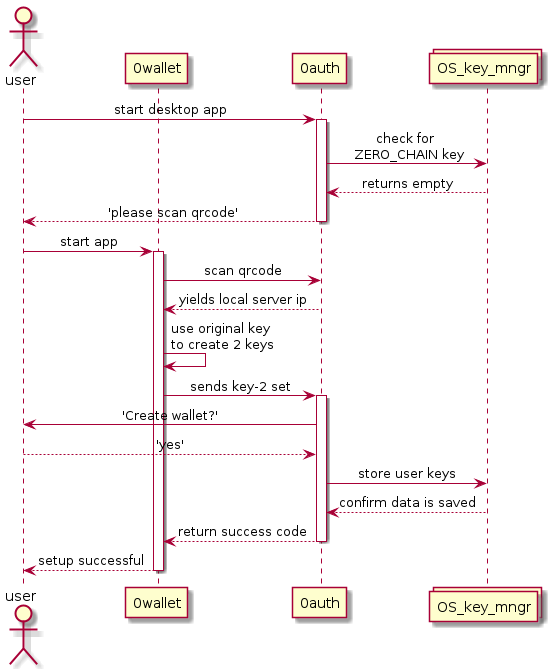
\includegraphics[width=\textwidth]{Images/setup_diagram.png}
\caption{Split Key Wallet Setup Process}
\label{fig:setup}
\end{figure}
\subsection{Transaction Signing Process}
Figure \ref{fig:transaction} depicts the transaction signing process using the split key wallet. When the user initiates a transaction from the mobile wallet, it is first signed with Key-1 stored on the mobile device. The partially signed transaction is then sent to the desktop application (0auth) for the second signature.
The user is prompted to confirm the transaction details on the desktop application. Upon confirmation, the transaction is signed with Key-2 stored securely in the desktop environment. The fully signed transaction, now containing signatures from both the mobile and desktop components, is returned to the mobile wallet. After verifying the signatures, the mobile wallet sends the transaction to the 0chain network for processing. This two-factor authentication process adds an extra layer of security to the user's transactions.
\begin{figure}[h]
\centering
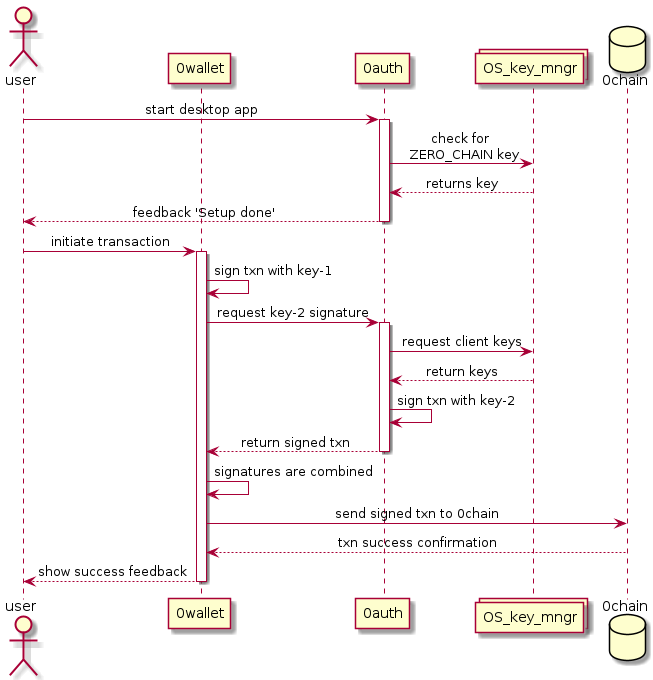
\includegraphics[width=\textwidth]{Images/transaction_diagram.png}
\caption{Split Key Wallet Transaction Signing Process}
\label{fig:transaction}
\end{figure}
\section{Integration Testing}
Rigorous integration testing is performed to ensure the smooth functioning of the split key wallet protocol and mobile authenticator within the Züs platform. The testing scenarios include:
\begin{itemize}
\item Key Generation and Splitting: Verifying the correctness of key generation and the splitting of the private key into multiple components.
\item Transaction Signing: Testing the end-to-end process of initiating a transaction, generating partial signatures, and combining them to produce the final signature.
\item Mobile Authenticator Functionality: Validating the mobile authenticator's user interface, biometric authentication, secure storage, and push notification capabilities.
\item Error Handling and Recovery: Testing various error scenarios, such as network disruptions or device failures, and ensuring proper error handling and recovery mechanisms are in place.
\end{itemize}
The implementation phase involves close collaboration between the development team and the Züs platform stakeholders to ensure seamless integration and adherence to the platform's security and performance requirements.
